\section{Model-View-ViewModel pattern} \label{sc:MVCVM}
The Model-View-ViewModel pattern (MVVM) is used to illuminate a clear distinction between the different components of the program, as well as allowing a complete seperation of the Views (UI) and the functionality within the program. An overview of MVVM can be seen on \autoref{fig:MVVM}. 
\par
The View part of MVVM handles the UI component of the system. The view component contains the logic directly related to connecting certain elements of the UI to the ViewModel component. In some cases the view file contains code related to directly manipulating or fetching data from the UI when the limitations of WPF binding is reached \citep{WPFandMVVM}.

\begin{figure}[H]
    \centering
    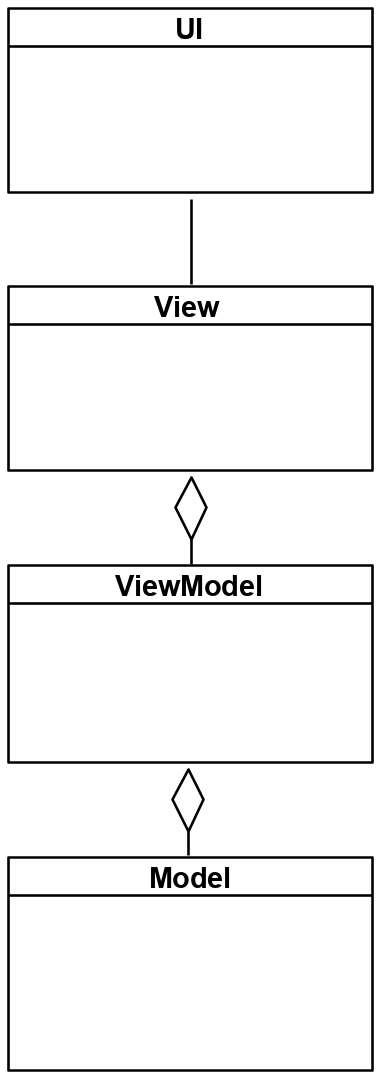
\includegraphics[width=0.2\textwidth]{figures/Implementation/MVVM.PNG}
    \caption{Model-View-ViewModel overview}
    \label{fig:MVVM}
\end{figure}

The next element in the structure seen on \autoref{fig:MVVM} is the view model component. This handles the conversion of data from the model layer to the view. The view model only contains the required logic to take the data presented in the model, and make it available to the view, as well as controlling the visibility of elements on the UI. The interaction between the UI and the view model is done by setting the \textit{DataContext} of the view, to point to the view model (see \autoref{code:AssetEditorView}). By setting the \textit{DataContext} the WPF framework can bind to the public properties within the view model. \citep{WPFandMVVM}

\begin{listing}[H]
\begin{minted}[frame=lines, framesep=3mm, baselinestretch=1, linenos, bgcolor=LightGray, escapeinside='', breaklines]{csharp}

public AssetEditor(IAssetController assetController, ITagListController tagListController)
{
    InitializeComponent();
    DataContext = new AssetEditorViewModel(assetController, tagListController);
}

\end{minted}
\captionof{listing}{AssetEditor.xaml.cs Example.}
\label{code:AssetEditorView}
\end{listing}

Most pages contain complicated functionality that would clutter the view model with methods that does not directly change information on the view. In these cases a controller class has been introduced in between the model and view model classes (see \autoref{sc:function_component}). The controllers contains functions related to updating, saving, or deleting specific instances of models. 
\par
In the MVVM pattern, the business logic, such as the business rules and the data access, should be in the model \citep{MvvmBasics}. In order to have a separation of concerns, these functionalities have been distributed to several different components, each with their own responsibility. Among these are the repositories (see \autoref{sc:RepositoryPatern}) that are responsible for the data access, and the controllers (see \autoref{sc:Controllers}) that are responsible for using the repositories and manipulating the data from these.
\par
% The controllers are introduced in order to keep the models pure, in the sense that they contain relevant data, and little to no functionality. The controllers are inspired by the controller component from the Model-View-Controller (MVC) pattern. \todo[inline]{Er det nødvendigt at have med == ja ( Beskriv MVC med kilder)}
% It is also similar to the Service-Layer pattern. \todo[inline]{Beskriv relevante dele af service layer pattern, med kilder.}
% \par
Examples and further explanation of the different elements of MVVM are described later in this section.


% https://scottlilly.com/c-design-patterns-mvvm-model-view-viewmodel/
% https://intellitect.com/getting-started-model-view-viewmodel-mvvm-pattern-using-windows-presentation-framework-wpf/
